% \newpage \ \thispagestyle{empty} \newpage

\chapter{Motivazioni alla base del tirocinio}
\label{cap:motivazioni-tirocinio}
Questo capitolo discute le motivazioni che hanno portato al compimento del percorso di tirocinio curricolare, dal punto di vista aziendale (si propone quella che, a mio parere, è la visione di \textit{\textbf{Trizeta}}) e dal mio punto di vista,
descrivendo i vincoli, gli obiettivi e le esigenze che il progetto proposto punta a soddisfare.

\section{Strategia aziendale}

% In questa sezione descriverò il rapporto che l'azienda ha nei confronti dei tirocini (universitari e non) dal punto di vista delle tecnologie, dei prodotti, del mercato e dal punto di vista di investimento sulle risorse umane.
In base a quanto ho potuto osservare e capire durante il periodo di \textit{stage}, la strategia di gestione dei tirocini curricolari dell'azienda ospitante persegue i seguenti obiettivi:
\begin{itemize}
    \item \textbf{Innovazione}: come riportato al termine della sezione \hyperref[sec:innovazione]{§1.4}, l'\glslink{innovazione}{innovazione} (ovvero l'introduzione di miglioramenti e novità) negli strumenti e nelle tecnologie utilizzate, motivata da esigenze produttive o di mercato,
    può avvalersi (come nel mio caso) del parere motivato del tirocinante tenendo conto del grado di maturità e delle caratteristiche del lavoro svolto per \textit{testare} le novità da introdurre;
    \item \textbf{Integrazione di prodotti esistenti}: il parco \textit{software \textbf{Trizeta}} è vasto (in relazione alle dimensioni dell'azienda) ed eterogeneo e la clientela richiede spesso l'implementazione di nuove funzionalità per rispondere a nuove esigenze; un modo per eseguire
        una prima integrazione di tali funzionalità (in versione \textit{beta} o di \textit{proof of concept}) si basa sul lavoro di uno o più tirocinanti;
        \vspace{-20mm}
        \begin{figure}[H]
            \centering
            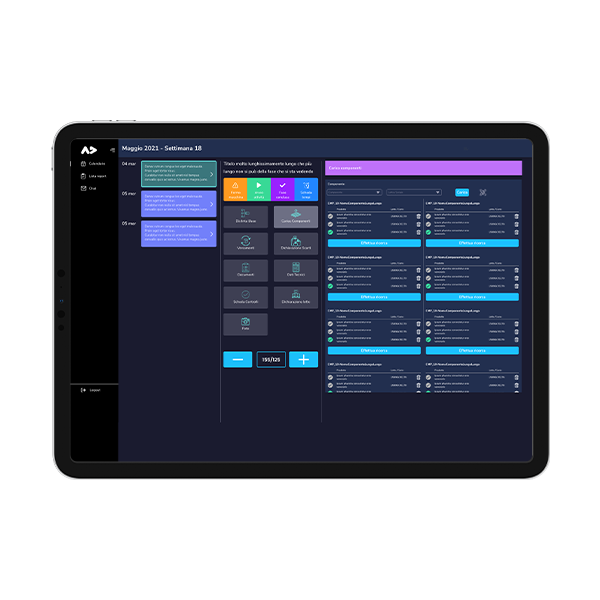
\includegraphics[width=0.8\textwidth]{images/ademes.png}
            \vspace{-20mm}
            \caption[Interfaccia del \textit{software ADeMES}]{Interfaccia del \textit{software ADeMES} \textit{\textbf{Trizeta}}\footnotemark}
        \end{figure}
        \footnotetext{Fonte: \href{https://trizeta.com/ade-mes/}{https://trizeta.com}}
    \item \textbf{Creazione di nuovi prodotti}: è possibile che la risposta alle nuove esigenze della clientela non sia possibile direttamente all'interno dei prodotti già esistenti (per separazione di ambito o
        per non compromettere la mantenibilità dei prodotti esistenti): in questo caso, concordando lo \glslink{tech-stack}{\textit{stack} tecnologico} (l'insieme delle tecnologie) da usare, ho potuto implementare un prodotto prototipale \textit{ex-novo} in base alle indicazioni ricevute;
    \item \textbf{Valutazione delle competenze} del tirocinante: il periodo di tirocinio è occasione di introduzione del tirocinante nel contesto aziendale e, per quanto riguarda la mia esperienza, formazione sulla visione aziendale, sui processi in atto, sulle tecnologie utilizzate
        e sulle abilità richieste per l'esecuzione delle attività lavorative; l'azienda ospitante fornisce quindi una formazione di base e valuta quali sono le reazioni agli stimoli (lavorativi e non) in funzione dell'inserimento del tirocinante nel \textit{team} aziendale.
        \begin{figure}[H]
            \centering
            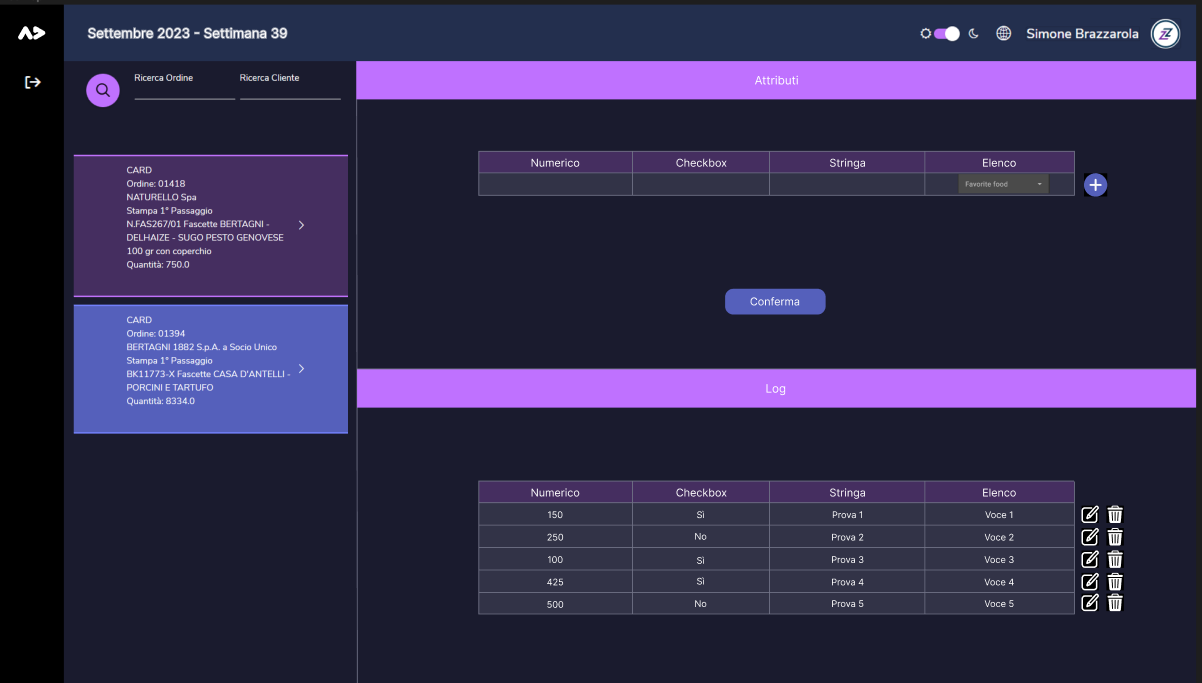
\includegraphics[width=0.8\textwidth]{images/dashboard.png}
            \caption[Interfaccia del prodotto \textit{ADeQA}]{Interfaccia del prodotto \textit{ADeQA}, oggetto del tirocinio}
        \end{figure}
\end{itemize}
\section{Problematiche poste in essere}

% In questa sezione descriverò quali problemi, a livello macroscopico, il prodotto \textit{software} da me sviluppato ha consentito di superare.
Scopo delle mie attività di \textit{stage} è la creazione di una \glslink{pwag}{\textit{Progressive Web App}}, ovvero un'applicazione \textit{web} che mette a disposizione funzionalità aggiuntive rispetto a quelle offerte da un sito \textit{web} (ad esempio, la fruizione dei servizi anche in modalità \textit{offline}) per la raccolta di dati relativi al controllo della qualità delle linee produttive di aziende manifatturiere. \\
Ogni linea produttiva è costituita da un insieme di "fasi" di lavorazione: ogni fase di lavorazione è considerabile come una \textit{black-box}\footnote{\gls{black-box}}, ovvero un processo di cui si conoscono gli \textit{input} (materia prima o semilavorati in ingresso)
e gli \textit{output} (semilavorati o prodotti finiti) ma non il funzionamento interno.
\begin{figure}[H]
    \centering
    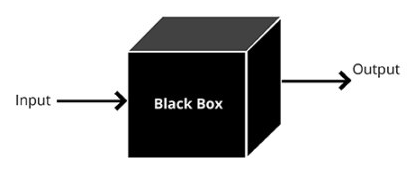
\includegraphics[width=0.6\textwidth]{images/black-box.png}
    \caption[Schema sintesi del concetto di \textit{black-box}]{Schema sintesi del concetto di \glslink{black-box}{\textit{black-box}} \footnotemark}
\end{figure}
\footnotetext{Fonte: \href{https://www.quora.com/Machine-learning-classifier-is-a-black-box-Why-does-everyone-still-use-it-1}{https://www.quora.com}}
Ogni fase è associata a un insieme di caratteristiche (dette "attributi") relative ai prodotti in uscita dalla stessa: esse sono di interesse per comprendere se la lavorazione ha prodotto articoli utilizzabili nelle fasi successive / nello stoccaggio degli stessi o meno. \\
Non è noto a priori il numero nè il tipo di attributi associati a una determinata fase di lavorazione: sono tutte informazioni ottenibili tramite l'utilizzo di servizi \textit{backend}\footnote{\gls{backend}} (relativi alla struttura ed alla logica di persistenza) esposti dal \textit{tutor} aziendale con una
serie di \textit{API\footnote{\gls{apig}} REST\footnote{\gls{restg}}} (astrazioni che consentono di eseguire operazioni sui dati di dominio in una architettura \textit{client - server}, con la possibilità di salvare le risposte ottenute, senza memorizzare lo stato del \textit{software} \textit{client}). \\
L'obiettivo del prodotto è consentire all'utente (operatore in linea di produzione) di inserire, modificare, eliminare e visualizzare dati di controllo qualità per le fasi desiderate (in gergo tecnico, eseguire le operazioni \textit{CRUD}, ovvero \textit{"Create", "Read", "Update" e"Delete"}, sui dati di qualità).

\section{Obiettivi}
\label{sec:obiettivi-aziendali}
Riporto le notazioni utilizzate in seguito per identificare gli obiettivi delle attività:
\begin{itemize}
    \item \textbf{O} per i requisiti obbligatori, vincolanti in quanto obiettivo primario richiesto dal committente;
    \item \textbf{D} per i requisiti desiderabili, non vincolanti o strettamente necessari, ma dal riconoscibile valore aggiunto;
    \item \textbf{F} per i requisiti facoltativi, rappresentanti valore aggiunto non strettamente competitivo.
\end{itemize}
Le sigle precedentemente indicate saranno seguite da una coppia sequenziale di numeri, identificativo del requisito. \\
Di seguito, la lista degli obiettivi di tirocinio:
\begin{itemize}
    \item \textbf{Obbligatori}
        \begin{itemize}
            \item \textbf{O01}: comprensione dei requisiti utente da soddisfare;
            \item \textbf{O02}: studio dell'interfaccia dell'applicazione \textit{ADeMES}, che verrà integrata con il prodotto da sviluppare durante il tirocinio; %mettere la tabella
            \item \textbf{O03}: acquisizione della sufficiente dimestichezza con i concetti di base del \textit{framework Angular}; %sezione 3.4.3 architettura
            \item \textbf{O04}: progettazione dell'interfaccia grafica in base allo stile dell'interfaccia dell'applicazione \textit{ADeMES}; %sezione 3.4.2
            \item \textbf{O05}: sviluppo di una versione di base dell'applicazione \textit{web} che consenta di eseguire le operazioni \textit{CRUD} sui dati di qualità; %validazione
            \item \textbf{O06}: \textit{live demo} della web application in un ambiente simulato; %validazione
            \item \textbf{O07}: studio e scelta (motivata) della tecnologia per la fruizione dell'applicazione in lingua inglese; %sezione 3.4.1
            \item \textbf{O08}: il \textit{software} deve potersi integrare nel \textit{software} ADeMES mediante un elemento \texttt{<iframe>} \textit{HTML}; %post-message nella stessa sezione
            \item \textbf{O09}: il \textit{software} deve poter essere eseguibile in modalità \textit{standalone}\footnote{\gls{standalone}} (in questo caso, in grado di funzionare anche senza l'ausilio del \textit{software ADeMES}). %sezione 3.8.2
        \end{itemize}
    \item \textbf{Desiderabili}
        \begin{itemize}
            \item \textbf{D01}: ottimizzazione dei servizi esposti. %nope, motivare
        \end{itemize}
    \item \textbf{Facoltativi}
        \begin{itemize}
            \item \textbf{F01}: ottimizzazione dell'esperienza utente per compatibilità con \textit{ADeMES}; %validazione
            \item \textbf{F02}: ottimizzazione dell'interfaccia grafica, per rendere quanto più simile il prodotto a \textit{ADeMES}; %tabella di O02
            \item \textbf{F03}: possibilità di fruizione dell'applicazione in lingua spagnola. %sezione 3.4.1
        \end{itemize}
\end{itemize}



\section{Vincoli}

% In questa sezione descriverò (entrando nei particolari, rispetto alla sezione precedente) le condizioni imposte ed i risultati prefissati.
Il progetto si focalizza sullo sviluppo di codice relativo all'interfaccia grafica e questo aspetto caratterizza le condizioni imposte per lo svolgimento del lavoro e le aspettative sul risultato:
\begin{itemize}
    \item Il prodotto deve essere sviluppato usando il \textit{framework Angular} alla versione 16;
    \item Il prodotto deve essere una \glslink{pwag}{\textit{Progressive Web App}} (applicazione \textit{web} installabile come se fosse un'applicazione nativa);
    \item Il prodotto deve fare uso delle \glslink{apig}{API} messe a disposizione da \textit{\textbf{Trizeta}}, ovvero delle regole di comunicazione tra \glslink{frontend}{\textit{frontend}} (interfaccia grafica) e \glslink{backend}{\textit{backend}} (\textit{software} di modellazione e memorizzazione dei dati di dominio);
    \item Il prodotto deve essere utilizzabile dagli operatori di linea produttiva tramite dispositivi mobili (obbligatoriamente tramite \textit{tablet}, facoltativamente tramite \textit{smartphone});
    \item Deve essere redatto un manuale utente che  descriva interfaccia grafica ed esperienza utente del \textit{software} sviluppato.
\end{itemize}

\section{Pianificazione}
\label{sec:pianificazione}
Ho rispettato la pianificazione delle attività, redatta anticipatamente rispetto all'inizio del progetto e disponibile di seguito, per la maggior parte del tempo richiesto dalle attività di tirocinio: solamente l'interfacciamento coi servizi
di scrittura dati è avvenuto in ritardo, data l'assenza temporanea degli stessi.

\begin{itemize}
    \item \textbf{Prima Settimana (40 ore)}
    \begin{itemize}
        \item Incontro con persone coinvolte nel progetto per discutere i requisiti e le richieste relativamente al sistema da sviluppare;
        \item Verifica credenziali e strumenti di lavoro assegnati;
        \item Presa visione dell’infrastruttura esistente;
        \item Formazione sulle tecnologie adottate.
    \end{itemize}
    \item \textbf{Seconda Settimana - (40 ore)} 
    \begin{itemize}
        \item Analisi e mappatura dei servizi esistenti;
        \item Documentazione dell'analisi dei servizi esposti.
    \end{itemize}
    \item \textbf{Terza Settimana - (40 ore)} 
    \begin{itemize}
        \item Analisi interfaccia/esperienza utente della \textit{web application};
        \item Documentazione dell'analisi dell'interfaccia della \textit{web application};
        \item Preparazione di un prototipo dimostrativo.
    \end{itemize}
    \item \textbf{Quarta Settimana - (40 ore)} 
    \begin{itemize}
        \item Scelta della tecnologia e del \textit{framework} da utilizzare;
        \item Conclusione della documentazione di analisi;
        \item Documentazione delle scelte progettuali;
        \item Predisposizione infrastruttura della \textit{web application}.
    \end{itemize}
    \item \textbf{Quinta Settimana - (40 ore)} 
    \begin{itemize}
        \item Documentazione delle scelte progettuali;
        \item Sviluppo \textit{web application} ed interfacciamento con i servizi di lettura dati esposti.
    \end{itemize}
    \item \textbf{Sesta Settimana - (40 ore)} 
    \begin{itemize}
        \item Conclusione della documentazione delle scelte progettuali;
        \item Sviluppo \textit{web application} ed interfacciamento con i servizi di scrittura dati esposti.
    \end{itemize}
    \item \textbf{Settima Settimana - (40 ore)} 
    \begin{itemize}
        \item Collaudo dell'applicazione;
        \item \textit{Test} e correzione degli eventuali errori;
        \item Stesura della documentazione finale.
    \end{itemize}
    \item \textbf{Ottava Settimana - Conclusione (40 ore)} 
    \begin{itemize}
        \item Conclusione del collaudo dell'applicazione;
        \item Conclusione \textit{test} e correzione degli eventuali errori;
        \item Conclusione della stesura della documentazione finale.
    \end{itemize}
\end{itemize}

Di seguito, la distribuzione delle ore lavorative in relazione alle macro-attività:
    \begin{table}[H]
        \begin{tabularx}{\textwidth}{|c|X|}
            \hline
            \textbf{Durata in ore} & \textbf{Descrizione dell'attività} \\ \hline
            
            \textbf{40} & \textbf{Formazione sulle tecnologie} \\	 
            \hline
            
            \textbf{200} & \textbf{Definizione architettura di riferimento e relativa documentazione} \\ \hdashline 
            \multirow{3}{0cm}\\ 
            & 
            {Analisi del problema e del dominio applicativo} \\
            & 
            {Progettazione della piattaforma e relativi \textit{test}} \\
            & 
            {Stesura documentazione relativa ad analisi e progettazione} \\
            \hline
            
            \textbf{80} & \textbf{Collaudo Finale}  \\ \hdashline 
            \multirow{4}{0cm}\\ 
            & 
            {Collaudo} \\
            & 
            {Stesura documentazione finale} \\
            & 
            {Incontro di presentazione della piattaforma con gli \glslink{stakeholder}{\textit{stakeholders}}} \\
            & 
            {\textit{Live demo} di tutto il lavoro di \textit{stage}} \\
            \hline
            
            \textbf{Totale ore} & \multicolumn{1}{|c|}{\textbf{320}} \\ \hline
        \end{tabularx}
        \caption{Distribuzione delle ore di lavoro}
    \end{table}
    \vspace{0.5cm}
    Riporto di seguito il diagramma di \textit{Gantt} relativo al piano di lavoro previsto.
    \begin{figure}[H]
        \makebox[\textwidth][c]{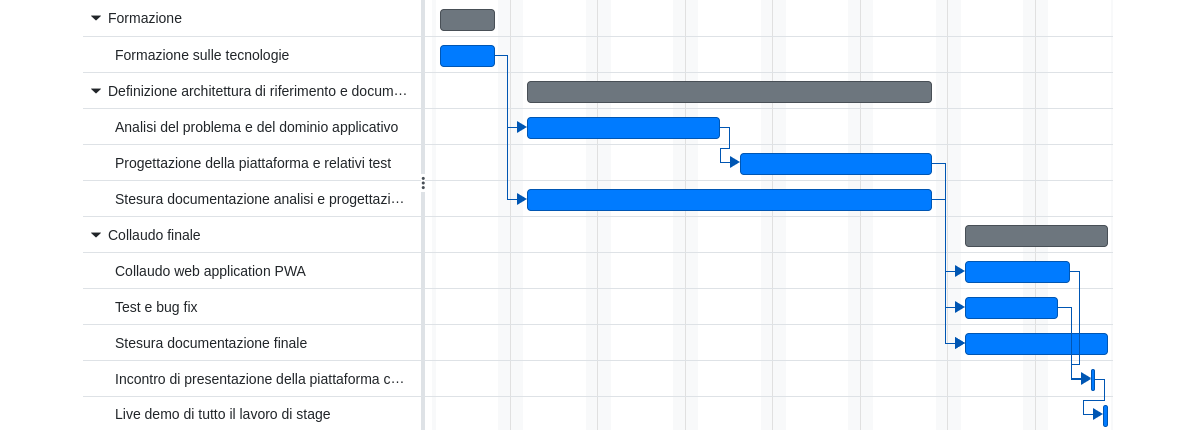
\includegraphics[width=1.15\textwidth]{images/gantt5.png}}
        \caption[Diagramma di \textit{Gantt} di suddivisione delle attività]{Diagramma di \textit{Gantt} di suddivisione delle attività}
    \end{figure}


\section{Scelta del tirocinio}
% In questa sezione descriverò le motivazioni che mi hanno portato a scegliere il progetto di tirocinio curricolare, indicando punti a favore e punti a sfavore a monte della scelta.
Le ragioni che mi hanno portato a scegliere il progetto di tirocinio curricolare offerto da \textit{\textbf{Trizeta}} possono essere così schematizzate:
\begin{itemize}
    \item \textbf{Introduzione al mondo del lavoro (ambito informatico)}: nonostante i tirocini curricolari sostenuti nel corso della mia carriera scolastica, prima di questo \textit{stage} non avevo mai avuto occasione di lavorare in ambito informatico, 
            probabilmente per timore di non essere in grado di affrontare le sfide dello sviluppo di prodotti \textit{software};
    \item \textbf{Desiderio di conoscenza di una realtà locale}: avendo frequentato un istituto di istruzione superiore limitrofo alla sede aziendale, ho sempre sentito nominare \textit{\textbf{Trizeta}} dai docenti e dai compagni di studi dato il suo 
        coinvolgimento in attività didattiche organizzate dall'istituto scolastico;
    \item \textbf{Curiosità per lo sviluppo \textit{frontend}}: nel corso della mia esperienza universitaria, la progettazione e la realizzazione di interfacce grafiche sono state piuttosto scarne e non si sono mai confrontate con vere e proprie
        richieste da parte di utenti finali o persone interessate nella buona riuscita del progetto (\glslink{stakeholder}{\textit{stakeholders}}) che avessero ben chiari i bisogni e le esigenze a cui dare risposta.
\end{itemize}

\begin{figure}[H]
    \centering
    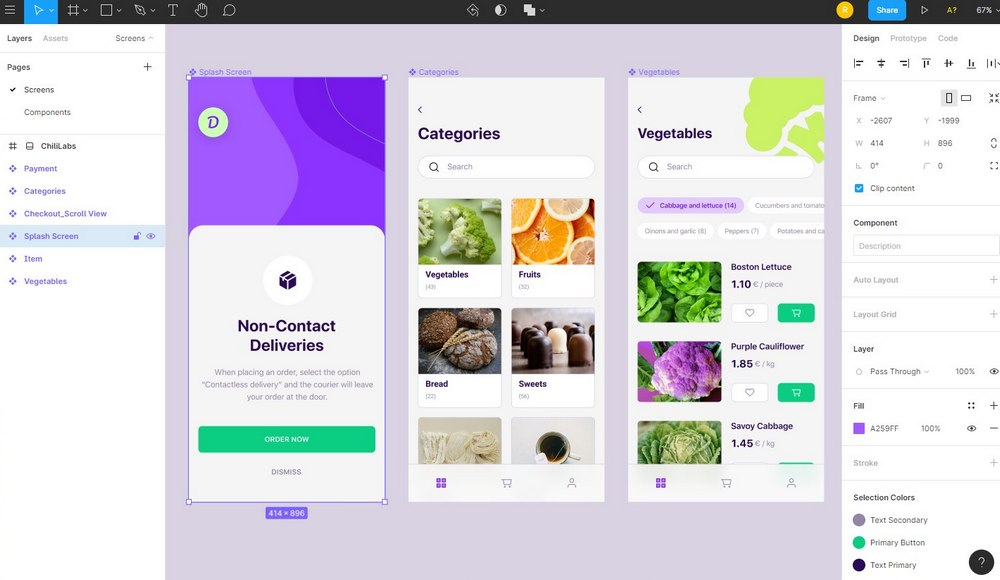
\includegraphics[width=0.8\textwidth]{images/figma-editor.jpg}
    \caption[Interfaccia del \textit{software Figma}]{Interfaccia del \textit{software Figma}, usato per la progettazione dell'interfaccia utente\footnotemark}
\end{figure}
\footnotetext{Fonte: \href{https://www.toponseek.com/blogs/figma-la-gi/}{https://www.toponseek.com}}
\label{sec:obiettivi-personali}
Queste motivazioni (ed il contesto personale in cui ho svolto le attività lavorative) mi hanno consentito di definire una serie di obiettivi personali per quanto riguarda la scelta dell'azienda, il tema delle attività e l'acquisizione di conoscenze e competenze:
\begin{itemize}
    \item Capire come convertire una \textit{web application} in una \glslink{pwa}{\textit{Progressive Web App}}, ovvero un'applicazione che coniuga caratteristiche di un'applicazione nativa (quali l'installazione e l'aspetto grafico) e caratteristiche di un'applicazione \textit{web} (come la possibilità di utilizzo tramite \textit{browser});
    \item Sviluppare un'interfaccia grafica che si adatti a \textit{desktop}, \textit{tablet} e \textit{smartphone};
    \item Comprendere come rendere fruibile in più lingue un prodotto \textit{software};
    \item Capire come si possono gestire diversi temi grafici (tipicamente identificati come "tema chiaro" e "tema scuro") in un'interfaccia grafica \textit{web};
    \item Ideare un prodotto in grado di integrarsi con successo in un \textit{software} già esistente.
\end{itemize}